\documentclass[letterpaper,11pt]{article}
% Soporte para los acentos.
\usepackage[utf8x]{inputenc}
\usepackage[T1]{fontenc}    
% Idioma español.
\usepackage[spanish,mexico, es-tabla]{babel}
% Soporte de símbolos adicionales (matemáticas)
\usepackage{multirow}
\usepackage{amsmath}		
\usepackage{amssymb}		
\usepackage{amsthm}
\usepackage{amsfonts}
\usepackage{latexsym}
\usepackage{enumerate}
\usepackage{ragged2e}
% Soporte para la imágenes.
\usepackage{graphicx}
% Modificamos los márgenes del documento.
\usepackage[lmargin=2cm,rmargin=2cm,top=2cm,bottom=2cm]{geometry}

\title{Universidad Nacional Autónoma de México \\
       Facultad de Ciencias \\
       Estructuras Discretas \\ 
       Tarea 3}
\author{Rubí Rojas Tania Michelle \\
        taniarubi@ciencias.unam.mx \\
        \# cuenta: 315121719}
\date{3 de noviembre de 2017}

\begin{document}
\maketitle

\begin{enumerate}
    % Ejericicio 1.
    \item Demuestre que cada una de las siguientes fórmulas se cumple para cada
    $n \in ℕ$.
    \begin{itemize}
        % Ejercicio 1.1
        \item[a)] $∑_{i=1}^{n}(2i -1)^{3} = n^{2}(2n^{2}-1)$
        \begin{proof}
            Inducción sobre $n$.
            \begin{itemize}
                \item Base de inducción. \\
                n = 1. Este caso se cumple ya que 

                $∑_{i=1}^{1}(2i - 1)^{3} = (2(1) - 1)^{3} = (1)^{3} = 1 = 
                1 (2(1) - 1) =(1)^{2}(2(1)^{2} - 1)$

                \item Hipótesis de inducción. \\
                Supongamos que el resultado es cierto para $n \geq 1$, es decir, 
                supongamos que se cumple $\sum_{i=1}^{n}(2i-1)^{3} = 
                n^{2}(2n^{2}-1)$.

                \item Paso inductivo. \\ 
                Tenemos que demostrar que la fórmula es válida para $n + 1$, es 
                decir, que se cumple $\sum_{i=1}^{n+1} (2i - 1)^{3} = 
                (n +1)^{2}(2(n + 1)^{2} - 1) = (n+1)^{2}(2n^{2} + 4n + 1)$. 

                Entonces 
                \begin{align*}
                    \sum_{i=1}^{n+1} 
                    &= \bigg (\sum_{i=1}^{n}(2i-1)^{3} \bigg) + (2(n+1) - 1)^{3} \\ 
                    &= (n^{2}(2n^{2} - 1)) + (2(n+1) - 1)^{3} 
                    && \text{por H.I.} \\ 
                    &= (2^{4} - n^{2}) + (8n^{3} + 12n^{2} + 6n + 1)
                    && \text{desarrolando términos} \\
                    &= 2^{4} + 8n^{3} + 11n^{2} + 6n +1
                    && \text{agrupando términos semejantes} \\ 
                    &= (n+1)^{2}(2n^{2} + 4n + 1)
                    && \text{factorizando}
                \end{align*}
            \end{itemize}
        \end{proof}

        % Ejercicio 1.2
        \item[b)] $∑_{i=0}^{n}\frac{i}{2^{i}} = 2 - \frac{n + 2}{2^{n}}$
        \begin{proof}
            Inducción sobre $n$. 

            \begin{itemize}
                \item Base de inducción. \\ 
                $n = 0$ Este caso se cumple ya que 

                $∑_{i=0}^{0} \frac{0}{2^{0}} = \frac{0}{1} = 0 =
                2 - 2 = 2 - \frac{2}{1}= 2 - \frac{0+2}{2^{0}}$

                \item Hipótesis de inducción. \\ 
                Supongamos que el resultado es válido para $n \geq 0$, es decir, 
                supongamos que se cumple $∑_{i=0}^{n}\frac{i}{2^{i}} = 
                2 - \frac{n + 2}{2^{n}}$.

                \item Paso inductivo. \\ 
                Tenemos que demostrar que la fórmula es válida para $n + 1$, es 
                decir, que se cumple $∑_{i=0}^{n+1} \frac{i}{2^{i}} = 
                2 - \frac{(n+1) + 2}{2^{n+1}} = 2 - \frac{n+3}{2^{n+1}}$

                Entonces 
                \begin{align*}
                    ∑_{i=0}^{n+1} \frac{i}{2^{i}}
                    &= \bigg (∑_{i=0}^{n}\frac{i}{2^{i}} \bigg ) + 
                    \bigg (\frac{n+1}{2^{n+1}} \bigg) \\ 
                    &= \bigg (2 - \frac{n+2}{2^{n}} \bigg) + 
                    \bigg (\frac{n+1}{2^{n+1}} \bigg) 
                    && \text{por H.I.} \\ 
                    &= 2 - \bigg(\frac{n+2}{2^{n}} + \frac{n+1}{2^{n+1}} \bigg)
                    && \text{asociatividad} \\ 
                    &= 2 - \bigg( \frac{2(n+2) - (n+1)}{2^{n+1}} \bigg)
                    && \text{resolviendo suma} \\ 
                    &= 2 - \bigg(\frac{2n + 4 - n + 1}{2^{n+1}} \bigg)
                    && \text{simplificando} \\ 
                    &= 2 - \bigg( \frac{n - 3}{2^{n+1}}\bigg)
                    && \text{simplificando}
                \end{align*}
            \end{itemize}
        \end{proof}
    \end{itemize}

    % Ejercicio 2.
    \item Demuestre cada una de las siguientes desigualdades para los valores
    de $n \in ℕ$ especificados.
    \begin{itemize}
        % Ejercicio 2.1
        \item $(1 + \frac{1}{n})^{n} < n$ para cada $n \in ℕ$ tal que $n \geq 3$
        % Ejercicio 2.2
        \item $7n < 2^{n}$ para cada $n \in ℕ$ tal que $n \geq 6$
    \end{itemize}

    % Ejercicio 3.
    \item Demuestre que 
    \begin{center}
        $∏_{i=2}^{n}(1 - \frac{1}{i^{2}}) = (1 - \frac{1}{2^{2}}) \times \cdots
        \times (1 - \frac{1}{n^{2}}) = \frac{n + 1}{2n}$
    \end{center}

    Para cada $n \in ℕ$ tal que $n \geq 2$.

    % Ejercicio 4.
    \item Sean $\{r_{i}\}_{i \in ℕ^{\times}}$ la sucesión definida por 
    $r_{1} = 1$, y $r_{n + 1} = 4r_{n} + 7$ para cada $n \in ℕ$. 
    Demuestre que $r_{n} = \frac{1}{3}(10 \cdot 4^{n - 1} - 7)$ para cada 
    $n \in ℕ^{\times}$. 

    % Ejercicio 5.
    \item Sean $\{b_{i}\}_{i \in ℕ}$ la sucesión definida por $d_{0} = 2, 
    d_{1} = 3, $ y $d_{n} = d_{n-1} \cdot d_{n-2}$ para cada $n \in ℕ$ tal que 
    $n \geq 3$. Encuentre una fórmula explícita para $d_{n}$, y demuestre por 
    inducción que su fórmula funciona.

    % Ejercicio 6.
    \item Sea \textit{spar(n)} la función definida como $span(n) = 2 + 4 + 6 +
    ⋯ + 2n$. Defina una implementación recursiva llamada $f(n)$ para la función 
    $spar(n)$. Demuestre que $f(n) = n(n + 1)$.

    % Ejercicio 7.
    \item Una cadena de caracteres es palíndroma si es de la forma $ww^{R}$ 
    donde $w^{R}$ es $w$ escrita de atrás hacia adelante, por ejemplo, $0110,
    abbbba, holaaloh$. Defina al conjunto de las cadenas palíndromas 
    recursivamente, y demuestre mediante inducción estructural, que todas las 
    cadenas palíndromas definidas tienen un número par de símbolos. 

    % Ejercicio 8.
    \item La función $snoc$ en listas se define como sigue:
    \begin{center}
        $snoc \; \; c[x_{1}, ⋯, x_{n}] = [x_{1}, ⋯, x_{n}, c]$
    \end{center}

    \begin{itemize}
        % Ejercicio 8.1
        \item[a)] De una implementación recursiva para $snoc$.
        % Ejercicio 8.2
        \item[b)] Demuestre, usando la definición recursiva, que:
        \begin{center}
            $snoc \; \; c \; (xs\_ys) = xs\_ (snoc \; \; c \; ys)$
        \end{center} 
    \end{itemize}

    % Ejercicio 9.
    \item Considere la siguiente función misteriosa $mist$
    \begin{center}
        $mist \; [] \; ys = ys$

        $mist \; (x : xs) \;  ys = mist \; xs \; (x : ys)$
    \end{center}

    \begin{itemize}
        % Ejercicio 9.1
        \item[a)] ¿Qué hace la función $mist$?
        \item[b)] Muestre que $rev \; xs = mist \; xs \; []$, con $rev$ la 
        operación reversa sobre cadenas definidas cómo sigue: 
        \begin{center}
            $rev \; [] = []$

            $rev \; (a : ls) = rev \; ls\_[a]$
        \end{center}
    \end{itemize}

    % Ejercicio 10.
    \item Sea $A$ una fórmula de la lógica proposicional cuyos únicos 
    conectivos son $\land, \lor \neg$. Definimos la fórmula dual de $A$, 
    denotada como $A_{D}$, intercambiando $\land$ por $\lor$, $\lor$ por 
    $\land$ y reemplazando a cada variable $p$ por su negación $\neg p$.
    Por ejemplo, $A = (r \lor q) \land \neg p$, $A_{D} = (\neg r \land \neg q)
    \lor \neg \neg p$.
    \begin{itemize}
        % Ejercicio 10.1
        \item Defina recursivamente una función dual tal que $dual(A) = A_{D}$.
        % Ejercicio 10.2
        \item Muestre que $\neg A \equiv A_{D}$ mediante inducción sobre 
        fórmulas.
    \end{itemize}

    % Ejercicio 11.
    \item Resuelva los siguientes incisos para árboles binarios.
    \begin{itemize}
        % Ejercicio 11.1
        \item Defina recursivamente una función $hmi(T)$ que devuelve la hoja
        más a la izquierda en un árbol binario.
        % Ejercicio 11.2
        \item La distancia entre la raíz $r$ de un árbol binario T hacía algún
        otro nodo $p$ es el número de aristas (líneas) que hay entre ambos nodos
        y la altura o profundidad de un árbol se define como la máxima distancia
        entre la raíz y alguna hoja más $1$. Demuestre que el número máximo de 
        hojas en un árbol de altura $n$ es $2^{n - 1}$.
        % Ejercicio 11.3
        \item De una definición recursiva que devuelva en una lista el recorrido
        post-orden de los árboles binarios. Si se tiene el siguiente árbol T, 
        el resultado del recorrido es el siguiente:
        \begin{center}
            \centerline{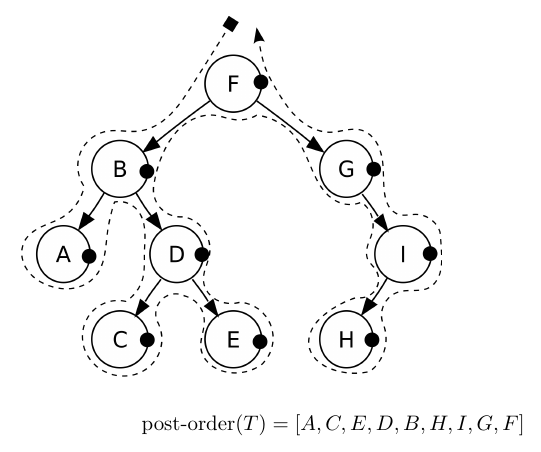
\includegraphics[scale=0.7]{recorrido.png}}
        \end{center}    
    \end{itemize}
\end{enumerate}
\end{document}
